%% ---------------------------------------------------------------------------
%% Measuring Retrieval-Layer Defense for RAG Agents
%% Prepared for Transactions on Machine Learning Research (TMLR)
%%
%% Requires tmlr.sty from https://github.com/JmlrOrg/tmlr-style-file
%%   \usepackage{tmlr}              -> anonymous submission version (default)
%%   \usepackage[preprint]{tmlr}    -> arXiv preprint with author names
%%   \usepackage[accepted]{tmlr}    -> camera ready
%% ---------------------------------------------------------------------------
\documentclass{article}
\usepackage{tmlr}

\usepackage{booktabs}
\usepackage{multirow}
\usepackage{amsmath,amssymb}
\usepackage{algorithm}
\usepackage{algpseudocode}
\usepackage{graphicx}
\usepackage{microtype}
\usepackage{xcolor}
\usepackage{url}

%% ---------------------------------------------------------------------------
%% Every numeric result in the prose comes from results_macros.tex, which NB6
%% generates from the experiment artifacts. Nothing is typed by hand. Until the
%% notebooks have been run, each macro renders as a visible red placeholder, so
%% an unfilled number cannot be mistaken for a real one.
%% ---------------------------------------------------------------------------
\providecommand{\PENDING}[1]{\textcolor{red}{\textbf{[#1]}}}
\IfFileExists{results_macros.tex}{%% Auto-generated by NB6. Do not edit by hand.
%% Regenerate by re-running NB6 after the experiment notebooks.
\newcommand{\alphaRtwo}{0.096}
\newcommand{\asrDoneAdaptive}{100.0\%}
\newcommand{\asrDoneStatic}{0.0\%}
\newcommand{\asrDthreeAdaptive}{68.3\%}
\newcommand{\complianceRate}{1\%}
\newcommand{\flatFrac}{40\%}
\newcommand{\headroomPct}{0\%}
\newcommand{\nBeirCorpora}{6}
\newcommand{\nBeirDocs}{272,117}
\newcommand{\nBeirQueries}{3,727}
\newcommand{\ndcgDenseCE}{0.438}
\newcommand{\ndcgFixed}{0.509}
\newcommand{\ndcgLearnedCE}{0.441}
\newcommand{\ndcgOracle}{0.575}
\newcommand{\overstatement}{68.7}
\newcommand{\promptHardenASR}{3.8\%}
\newcommand{\utilityCost}{0.0054}
}{%
  \newcommand{\ndcgDenseCE}{\PENDING{nDCG dense+CE}}
  \newcommand{\ndcgLearnedCE}{\PENDING{nDCG learned+CE}}
  \newcommand{\ndcgOracle}{\PENDING{nDCG oracle}}
  \newcommand{\ndcgFixed}{\PENDING{nDCG fixed alpha}}
  \newcommand{\headroomPct}{\PENDING{\% headroom captured}}
  \newcommand{\flatFrac}{\PENDING{\% flat queries}}
  \newcommand{\alphaRtwo}{\PENDING{alpha CV R2}}
  \newcommand{\asrDoneStatic}{\PENDING{D1 vs A0}}
  \newcommand{\asrDoneAdaptive}{\PENDING{D1 vs A5}}
  \newcommand{\asrDthreeAdaptive}{\PENDING{D3 vs A5}}
  \newcommand{\complianceRate}{\PENDING{P(comply|entry)}}
  \newcommand{\overstatement}{\PENDING{overstatement factor}}
  \newcommand{\utilityCost}{\PENDING{nDCG cost at 1\% FPR}}
  \newcommand{\promptHardenASR}{\PENDING{hardened-prompt ASR}}
  \newcommand{\nBeirCorpora}{\PENDING{n}}
  \newcommand{\nBeirDocs}{\PENDING{n docs}}
  \newcommand{\nBeirQueries}{\PENDING{n queries}}
}

\title{Measuring Retrieval-Layer Defense for Retrieval-Augmented Agents:\\
Adaptive Adversaries, Downstream Compliance, and the Limits of Learned Fusion}

\author{\name Anonymous \email anonymous@example.com \\
        \addr Anonymous Institution}

\def\month{01}
\def\year{2026}
\def\openreview{\url{https://openreview.net/forum?id=XXXXXXXXXX}}

\begin{document}
\maketitle

%% ===========================================================================
\begin{abstract}
%% ===========================================================================
Retrieval-augmented agents expose a security boundary at the retrieval layer:
any document the agent can retrieve can carry instructions. A natural response
is to filter retrieved documents before they enter the context window, and a
growing number of systems do. We ask what that filtering actually buys, and
report a measurement study whose main findings are corrective.

We evaluate a representative retrieval stack --- dense retrieval, BM25,
query-adaptive score fusion, cross-encoder reranking, and a lightweight
adversarial filter --- under three protocols the literature usually omits:
full-corpus retrieval on \nBeirCorpora{} BEIR collections with matched
reranking budgets, an attacker ladder culminating in a black-box score-guided
adversary evaluated at matched false-positive budgets, and downstream
measurement of whether a local instruction-tuned model actually complies with
injected directives.

Three results follow. First, \emph{query-adaptive fusion does not help}. An
oracle that selects the best fusion weight per query in hindsight reaches
\ndcgOracle{} nDCG@10 against \ndcgFixed{} for a single tuned global weight, so
headroom exists; a learned predictor captures \headroomPct{} of it. The reason
is identifiability, not model capacity: on \flatFrac{} of queries the entire
fusion-weight grid moves nDCG@10 by less than $0.01$, making the regression
target largely undefined ($R^2 = \alphaRtwo{}$ under cross-validation, including
for deliberately overpowered predictors). Second, \emph{lightweight filters do
not survive adaptive adversaries}. A three-feature filter of the kind commonly
deployed blocks static injection templates (ASR \asrDoneStatic{}) but fails
against an attacker allowed 200 queries to the detector (ASR
\asrDoneAdaptive{}), while a fine-tuned classifier at the same false-positive
budget holds at \asrDthreeAdaptive{}. Third, \emph{payload entry overstates
risk}. Conditioned on a payload reaching the context window, small
instruction-tuned models comply \complianceRate{} of the time, so the
retrieval-level metric used throughout this literature overstates exposure by
roughly \overstatement{}$\times$.

We recommend that retrieval-layer defenses be reported at matched
false-positive budgets, against at least one adaptive attacker, and alongside a
downstream compliance measurement. All code, generated attack corpora, and
per-query artifacts are released, along with a claim-audit script that ties
every number in this paper to the artifact that produced it.
\end{abstract}

%% ===========================================================================
\section{Introduction}
%% ===========================================================================

A retrieval-augmented agent \citep{lewis2020rag} reads documents it did not write. That is the point
of retrieval, and it is also the attack surface: an adversary who can place text
where the agent will retrieve it obtains a channel into the agent's context
window without touching model weights
\citep{greshake2023indirect,zou2024poisonedrag}. The threat is not
hypothetical --- injected tool descriptions redirect tool selection
\citep{shi2025toolhijacker}, and dynamic tool-discovery protocols widen the
surface further \citep{hou2025mcp}.

One response is to filter at the retrieval layer: score each retrieved document
for adversarial content and drop the suspicious ones before they reach the
model. This is attractive because it is cheap, model-agnostic, and does not
depend on the agent's instruction-following robustness. It is also increasingly
common. What is missing is a measurement of what it buys.

This paper supplies that measurement, and in doing so revisits two claims that
the retrieval-plus-defense literature --- including an earlier version of this
work --- has been making without adequate support.

\paragraph{Claim 1: query-adaptive fusion improves first-stage retrieval.}
Hybrid retrieval combines dense and lexical scores, usually with a fixed weight
or reciprocal rank fusion \citep{cormack2009rrf,bruch2023fusion}. The natural
refinement is to predict the weight per query. We find this does not work, and
--- more usefully --- we find out why. Section~\ref{sec:rq1} separates the two
possible explanations by measuring an oracle that picks the best weight per
query in hindsight. The oracle establishes real headroom, so the mechanism is
not vacuous in principle. But the per-query objective is nearly flat in the
fusion weight for most queries, which makes the regression target
ill-identified; a deliberately overpowered predictor does no better than a small
one, and neither beats a single tuned global weight.

\paragraph{Claim 2: retrieval-layer filtering substantially reduces attack
success.} Reported reductions in this literature are large --- often two orders
of magnitude. Section~\ref{sec:rq2} shows those numbers are an artifact of
evaluating against attackers who do not adapt. We construct a ladder of six
attackers, from static templates through a black-box score-guided adversary
with a bounded query budget, and evaluate six defenses against all of them at
\emph{matched false-positive budgets}. The lightweight three-feature filters
that dominate deployed systems collapse; classifiers fine-tuned on public
injection corpora largely hold. The gap between those two conclusions is
entirely invisible to a static evaluation, which is the methodological point.

\paragraph{An additional gap: the metric itself.} Nearly all retrieval-layer
security work, ours included, measures whether an adversarial document
\emph{entered} the retrieved set. What a practitioner needs to know is whether
the agent then \emph{did what the document said}. Section~\ref{sec:rq3}
measures both on identical episodes with real instruction-tuned models and
reports the ratio, which we call \emph{compliance given entry}. To our
knowledge this quantity has not previously been reported, and it is the factor
by which every payload-entry number in this literature --- ours included ---
must be discounted.

\paragraph{Relation to a prior version.} An earlier version of this work was
submitted to a conference venue and rejected. The reviews identified, correctly,
that its retrieval gains came from cross-encoder reranking rather than the
mechanism its title emphasised, that its main protocol reranked
dataset-provided candidate pools rather than retrieving from a corpus, and that
its security evaluation was too synthetic to support its claims. This paper is
not a rebuttal of those reviews; it accepts them and rebuilds the study around
what they imply. Appendix~\ref{app:changes} states every claim that changed and
why, so the two versions can be compared directly.

\paragraph{Contributions.}
\begin{enumerate}
\item A full-corpus evaluation of query-adaptive fusion on \nBeirCorpora{} BEIR
  collections under matched cross-encoder budgets, with an oracle upper bound
  that quantifies how much per-query weighting could win, and an identifiability
  analysis that explains why learning does not reach it
  (Section~\ref{sec:rq1}).
\item An attack $\times$ defense matrix over six attacker capability levels and
  six defenses, evaluated at matched false-positive budgets, including a
  black-box score-guided adversary under a stated query budget
  (Section~\ref{sec:rq2}).
\item The first measurement we know of relating retrieval-level payload entry to
  downstream behavioural compliance, on identical episodes, across model scales
  and context positions, together with a tool-selection loop
  (Section~\ref{sec:rq3}).
\item A reproducibility artifact that includes the generated attack corpora, all
  per-query scores, and a claim-audit script asserting that every number in this
  paper traces to a recorded artifact (Section~\ref{sec:repro}).
\end{enumerate}

%% ===========================================================================
\section{Background and related work}
%% ===========================================================================

\paragraph{Hybrid retrieval and fusion.} Dense retrieval \citep{karpukhin2020dpr}
is strong on paraphrase and weak on exact lexical match, motivating combination
with BM25. Reciprocal rank fusion \citep{cormack2009rrf} is the standard
rank-based method; convex combination of normalised scores is the standard
score-based one, and learned sparse representations such as SPLADE
\citep{formal2021splade} pursue the same goal by making the lexical channel
itself learnable. \citet{bruch2023fusion} analyse both and show that the choice
of normalisation and the value of the convex weight matter more than the choice
of fusion family, and that a well-tuned convex combination is a strong baseline
--- a finding our oracle analysis extends by bounding what \emph{per-query}
weighting could add on top. \citet{thakur2021beir} established BEIR as the
zero-shot retrieval benchmark we use, precisely so that retrieval claims are not
made on a single in-domain collection.

\paragraph{Reranking.} Cross-encoders \citep{nogueira2020passage} reliably
improve top-$k$ precision over any first stage, at a cost linear in the number
of reranked candidates. Because that improvement is large and largely
first-stage-agnostic, comparing a system that reranks against a baseline that
does not conflates the two effects. Our matched-budget grid
(Section~\ref{sec:protocol}) exists to prevent exactly this.

\paragraph{Prompt injection and RAG poisoning.} \citet{perez2022injection}
characterised prompt injection; \citet{greshake2023indirect} extended it to
indirect delivery through retrieved content. PoisonedRAG
\citep{zou2024poisonedrag} formalises knowledge-corruption attacks on RAG
corpora. \citet{liu2024formalizing} provide a benchmark and taxonomy of
injection attacks and defenses. AgentDojo \citep{debenedetti2024agentdojo} and
InjecAgent \citep{zhan2024injecagent} evaluate injection in full agent loops
with tool use, which is the setting our Section~\ref{sec:rq3} approximates at
smaller scale.

\paragraph{Defenses and the adaptive-evaluation problem.} Proposed defenses
include perplexity filtering \citep{alon2023detecting,jain2023baseline},
detector models, and training-time approaches such as StruQ
\citep{chen2024struq} and SecAlign \citep{chen2025secalign}. The methodological
hazard is well documented outside this literature:
\citet{athalye2018obfuscated} showed that most defenses accepted at a single
venue owed their apparent robustness to obfuscated gradients rather than to any
real security property, and \citet{carlini2019evaluating} and
\citet{tramer2020adaptive} generalised the lesson: a large majority of published
adversarial-example defenses lost most of their claimed robustness once attacks
were adapted to them. The retrieval-layer defense
literature is currently at the stage that literature was at before adaptive
evaluation became standard, and Section~\ref{sec:rq2} is an attempt to import
the practice rather than the conclusion.

\paragraph{Position effects.} \citet{liu2024lost} showed that a model's use of
retrieved context depends strongly on where in the context window the content
sits. We measure injection compliance as a function of the poison's rank for the
same reason: a security result at rank 0 does not transfer to rank 4.

\paragraph{Agent memory.} MemGPT \citep{packer2023memgpt}, MemoryBank
\citep{zhong2023memorybank}, and A-MEM \citep{xu2025amem} address persistent
agent memory. An earlier version of this work included a design for an episodic
memory graph. It is not part of this paper: nothing in our evaluation tests it,
and describing an unevaluated component alongside evaluated ones invites readers
to transfer confidence from one to the other. We note the direction here and
leave it to work that measures it.

%% ===========================================================================
\section{Study design}
\label{sec:protocol}
%% ===========================================================================

\subsection{System under test}

We study the retrieval stack in Figure~\ref{fig:pipeline}: a dense retriever, a
BM25 retriever, a fusion step, an optional cross-encoder reranker, and an
optional adversarial filter applied to the surviving list before it reaches the
model. This is not a proposal; it is the configuration deployed
retrieval-augmented systems converge on, and the object of measurement.

Dense retrieval uses \texttt{all-MiniLM-L6-v2} \citep{reimers2019sbert} by
default, with \texttt{bge-small-en-v1.5} \citep{xiao2023bge}, \texttt{gte-small},
and \texttt{e5-small-v2} \citep{wang2022e5} as generality checks. Lexical retrieval is BM25 with Lucene parameters
($k_1{=}0.9$, $b{=}0.4$), implemented with \texttt{bm25s} \citep{lu2024bm25s}.
Reranking uses \texttt{ms-marco-MiniLM-L-6-v2}. Retrieval is exact: dense search
is a normalised inner product computed by chunked matrix multiplication rather
than an approximate index, so no result depends on ANN parameters.

\paragraph{Fusion.} Given the top-$m$ lists from each channel, scores are
min--max normalised \emph{within the retrieved list}, and a document retrieved
by only one channel receives $0$ from the other. The fused score is
\begin{equation}
s(d) \;=\; \alpha\,\tilde{s}_{\text{dense}}(d) \;+\; (1-\alpha)\,\tilde{s}_{\text{lex}}(d).
\label{eq:fusion}
\end{equation}
We compare four policies for $\alpha$: reciprocal rank fusion as a
weight-free alternative; a single global $\alpha^\star$ tuned on a fitting set;
a per-query $\alpha$ predicted by a random forest from six query and
score-distribution features; and a per-query \emph{oracle} $\alpha$ chosen in
hindsight to maximise nDCG@10. The oracle is not a system. It is an upper bound
on any per-query fusion policy whatsoever, and it is what makes the learned
result interpretable.

Feature definitions, the exact normalisation convention, and the provenance of
the fitting queries are given in Appendix~\ref{app:features}; all three were
underspecified in the earlier version and are the kind of detail that determines
whether a hybrid-retrieval result reproduces.

\subsection{Threat model and attacker ladder}
\label{sec:threat}

The adversary controls text that enters the corpus --- web pages, documents, API
responses --- and has no access to model weights or to the agent's system
prompt. The adversary's goal is that a document it authored both (i) is
retrieved for a target query and (ii) causes the agent to follow a directive the
document contains. We instantiate that directive as emitting a fixed canary
token, which makes compliance unambiguous to score.

Attackers differ in what they know, summarised in Table~\ref{tab:attackers}.
The ladder is the design commitment of this paper: A0 and A1 are what the prior
literature evaluates, and A2--A6 are what an attacker who has read the defense
would do.

\begin{table}[t]
\centering
\small
\caption{Attacker capability ladder. Each level adds knowledge, not compute.
Every attacker must retain an immutable \emph{core directive} span, so evasion
cannot be achieved by weakening the payload; Section~\ref{sec:rq3} verifies on a
real model that the evaded documents still induce compliance.}
\label{tab:attackers}
\begin{tabular}{llll}
\toprule
& Attacker & Knows & Targets \\
\midrule
A0 & Static templates & nothing & --- \\
A1 & Query-conditioned & the target query & retrievability \\
A2 & Imperative-free paraphrase & the keyword list & keyword feature \\
A3 & Semantic camouflage & the corpus & centroid + query-similarity features \\
A4 & Length-matched & clean length statistics & length feature \\
A5 & Score-guided black box & query access to the detector & the deployed detector \\
A6 & Split payload ($k$ chunks) & the top-$k$ budget & per-document detection \\
\bottomrule
\end{tabular}
\end{table}

A5 is the adaptive attacker in the sense of \citet{tramer2020adaptive}. It is
permitted $B$ queries to the deployed detector and greedily accepts local edits
--- prepending genuine corpus text, synonym substitution on flagged tokens,
sentence reordering, filler insertion --- that lower the detection score,
subject to two hard constraints: the core directive survives verbatim, and
cosine similarity to the target query stays within $15\%$ of the unoptimised
payload's, so the document remains retrievable. No gradients and no model
internals are used; this is deliberately the weakest adaptive attacker we could
construct, which makes any failure it causes a lower bound on the true risk.

\subsection{Defense ladder}

Six defenses, each exposing a scalar suspicion score:
\textbf{D1}, a three-feature logistic classifier (clean-centroid cosine
similarity, imperative-keyword indicator, length ratio) trained on six clean and
six poison examples --- the configuration used in the prior version of this work
and, in our reading, representative of lightweight deployed filters;
\textbf{D1b}, the same three features trained on pooled public injection
corpora; \textbf{D2}, logistic regression on the full sentence embedding;
\textbf{D3}, a fine-tuned DistilBERT classifier; \textbf{D4}, an off-the-shelf
injection guard used zero-shot; \textbf{D5}, a windowed GPT-2 perplexity filter
in the style of \citet{alon2023detecting}; and \textbf{D6}, D3 combined with a
query-relevance heuristic. D1 versus D1b isolates \emph{small training set} from
\emph{weak features}, two defects that are otherwise conflated.

\subsection{Three protocol commitments}

\paragraph{Full-corpus retrieval.} Every retrieval number in this paper comes
from ranking a complete BEIR corpus (\nBeirDocs{} documents across
\nBeirCorpora{} collections, \nBeirQueries{} queries), scored with
\texttt{pytrec\_eval} \citep{vangysel2018pytreceval} so that nDCG@10
\citep{jarvelin2002ndcg} is directly comparable to published BEIR results. We do not rerank dataset-provided candidate pools anywhere.

\paragraph{Matched reranking budget.} Systems are compared only against systems
given the same number of cross-encoder forward passes. We report the grid over
budgets $\{0, 50, 100\}$ rather than a single configuration, because the
reranker dominates and a single configuration invites the comparison it is
meant to prevent.

\paragraph{Matched false-positive budget.} A defense's attack success rate is
meaningless without the false-positive rate at which it was measured. Every
defense's threshold is calibrated on held-out clean documents to hit a target
FPR in $\{0.1\%, 1\%, 5\%\}$, and every reported ASR names its operating point.

Statistical comparisons use a paired bootstrap over per-query scores
($10{,}000$ resamples) reporting mean differences with $95\%$ intervals and
effect sizes. We deliberately do not lead with $p$-values: at the query counts
involved, a paired test declares differences significant that are far below what
a practitioner would notice, and the earlier version of this work leaned on
$p < 10^{-100}$ for an effect of $0.028$.

%% ===========================================================================
\section{RQ1: Does query-adaptive fusion improve retrieval?}
\label{sec:rq1}
%% ===========================================================================

\subsection{Matched-budget comparison}

Table~\ref{tab:main_retrieval} reports nDCG@10 for every first stage at every
reranking budget. The pattern is unambiguous: at a fixed budget, all reasonable
first stages land within a narrow band, and the reranking budget moves results
far more than the choice of first stage does. Learned $\alpha$ with a
cross-encoder reaches \ndcgLearnedCE{} against \ndcgDenseCE{} for dense
retrieval with the same reranker.

\begin{table}[t]
\centering
\small
\caption{Full-corpus nDCG@10 on BEIR under a matched cross-encoder budget. Every first stage is scored at the same reranking depth, so the fusion mechanism is compared against dense retrieval on equal compute. Oracle $\alpha$ is an upper bound, not a system.}
\label{tab:main_retrieval}
\begin{tabular}{lccccccc}
\toprule
First stage & arguana & fiqa & nfcorpus & scidocs & scifact & trec-covid & Mean \\
\midrule
\multicolumn{8}{l}{\textit{no reranking}} \\
BM25 & 0.306 & 0.238 & 0.318 & 0.151 & 0.676 & 0.589 & 0.380 \\
Dense & 0.370 & 0.368 & 0.316 & 0.216 & 0.646 & 0.469 & 0.398 \\
RRF ($k{=}60$) & 0.368 & 0.374 & 0.342 & 0.199 & 0.715 & 0.698 & 0.449 \\
Fixed $\alpha^\star$ & 0.381 & 0.405 & 0.337 & 0.218 & 0.697 & 0.544 & 0.430 \\
Learned $\alpha$ & 0.359 & 0.366 & 0.358 & 0.189 & 0.727 & 0.692 & 0.449 \\
Learned $\alpha$ + dense override & 0.374 & 0.367 & 0.358 & 0.190 & 0.727 & 0.616 & 0.439 \\
\textit{Oracle} $\alpha$ & 0.440 & 0.480 & 0.404 & 0.264 & 0.782 & 0.774 & 0.524 \\
\midrule
\multicolumn{8}{l}{\textit{cross-encoder top-50}} \\
BM25 & 0.326 & 0.332 & 0.350 & 0.165 & 0.692 & 0.712 & 0.429 \\
Dense & 0.330 & 0.386 & 0.340 & 0.188 & 0.691 & 0.654 & 0.431 \\
RRF ($k{=}60$) & 0.326 & 0.372 & 0.356 & 0.172 & 0.695 & 0.751 & 0.445 \\
Fixed $\alpha^\star$ & 0.328 & 0.385 & 0.350 & 0.180 & 0.694 & 0.705 & 0.440 \\
Learned $\alpha$ & 0.327 & 0.370 & 0.354 & 0.170 & 0.695 & 0.749 & 0.444 \\
Learned $\alpha$ + dense override & 0.329 & 0.370 & 0.354 & 0.170 & 0.695 & 0.725 & 0.441 \\
\textit{Oracle} $\alpha$ & 0.327 & 0.379 & 0.359 & 0.177 & 0.702 & 0.758 & 0.450 \\
\midrule
\multicolumn{8}{l}{\textit{cross-encoder top-100}} \\
BM25 & 0.321 & 0.348 & 0.350 & 0.164 & 0.693 & 0.734 & 0.435 \\
Dense & 0.319 & 0.378 & 0.343 & 0.180 & 0.693 & 0.713 & 0.438 \\
RRF ($k{=}60$) & 0.316 & 0.370 & 0.356 & 0.169 & 0.691 & 0.742 & 0.441 \\
Fixed $\alpha^\star$ & 0.318 & 0.376 & 0.349 & 0.175 & 0.693 & 0.725 & 0.440 \\
Learned $\alpha$ & 0.316 & 0.367 & 0.353 & 0.169 & 0.693 & 0.745 & 0.441 \\
Learned $\alpha$ + dense override & 0.319 & 0.367 & 0.353 & 0.169 & 0.693 & 0.736 & 0.439 \\
\textit{Oracle} $\alpha$ & 0.319 & 0.374 & 0.357 & 0.173 & 0.694 & 0.756 & 0.445 \\
\bottomrule
\end{tabular}
\end{table}


This is the result the earlier version of this work reported as a $+2.80$
percentage point improvement. That figure came from comparing a reranked system
against unreranked baselines. Under a matched budget the gap largely
disappears, and what remains is attributable to the reranker.

\subsection{The oracle bound}

Whether per-query weighting is a bad idea or merely badly implemented is
settled by the oracle. Table~\ref{tab:alpha_policies} places every policy
against it.

\begin{table}[t]
\centering
\small
\caption{Per-query fusion policies against the oracle ceiling. ``\% headroom'' is the share of the oracle-minus-fixed gap a policy captures. Intervals are paired bootstrap over per-query nDCG@10.}
\label{tab:alpha_policies}
\begin{tabular}{lcccc}
\toprule
Policy & nDCG@10 & $\Delta$ vs.\ Dense & 95\% CI & \% headroom \\
\midrule
BM25 (alpha=0) & 0.3770 & -0.0792 & [-0.1007, -0.0576] & -199\% \\
Dense (alpha=1) & 0.4562 & +0.0000 & [+0.0000, +0.0000] & -79\% \\
RRF (k=60) & 0.4822 & +0.0260 & [+0.0105, +0.0418] & -40\% \\
Fixed alpha*=0.65 & 0.5089 & +0.0527 & [+0.0405, +0.0651] & 0\% \\
Oracle alpha (ceiling) & 0.5753 & +0.1192 & [+0.1061, +0.1327] & 100\% \\
Learned: RandomForest(50,d5) [CIKM config] & 0.4711 & +0.0149 & [-0.0022, +0.0324] & -57\% \\
Learned: RandomForest(500,d16) & 0.4731 & +0.0170 & [+0.0001, +0.0343] & -54\% \\
Learned: GradientBoosting(500) & 0.4675 & +0.0114 & [-0.0059, +0.0290] & -62\% \\
\bottomrule
\end{tabular}
\end{table}


Headroom exists: the oracle reaches \ndcgOracle{} against \ndcgFixed{} for the
best single global weight. Per-query weighting is therefore not vacuous. But the
learned predictor captures only \headroomPct{} of that gap.

\subsection{Why learning does not reach it}

Figure~\ref{fig:headroom} gives the explanation, and it is a property of the
objective rather than of the model. On \flatFrac{} of queries, sweeping $\alpha$
across its entire range moves nDCG@10 by less than $0.01$. For those queries the
oracle $\alpha^\star$ is whichever grid point won a tie, and a regressor trained
on them is fitting noise. The target is not merely hard to predict; on most
queries it is not defined.

\begin{figure}[t]
\centering
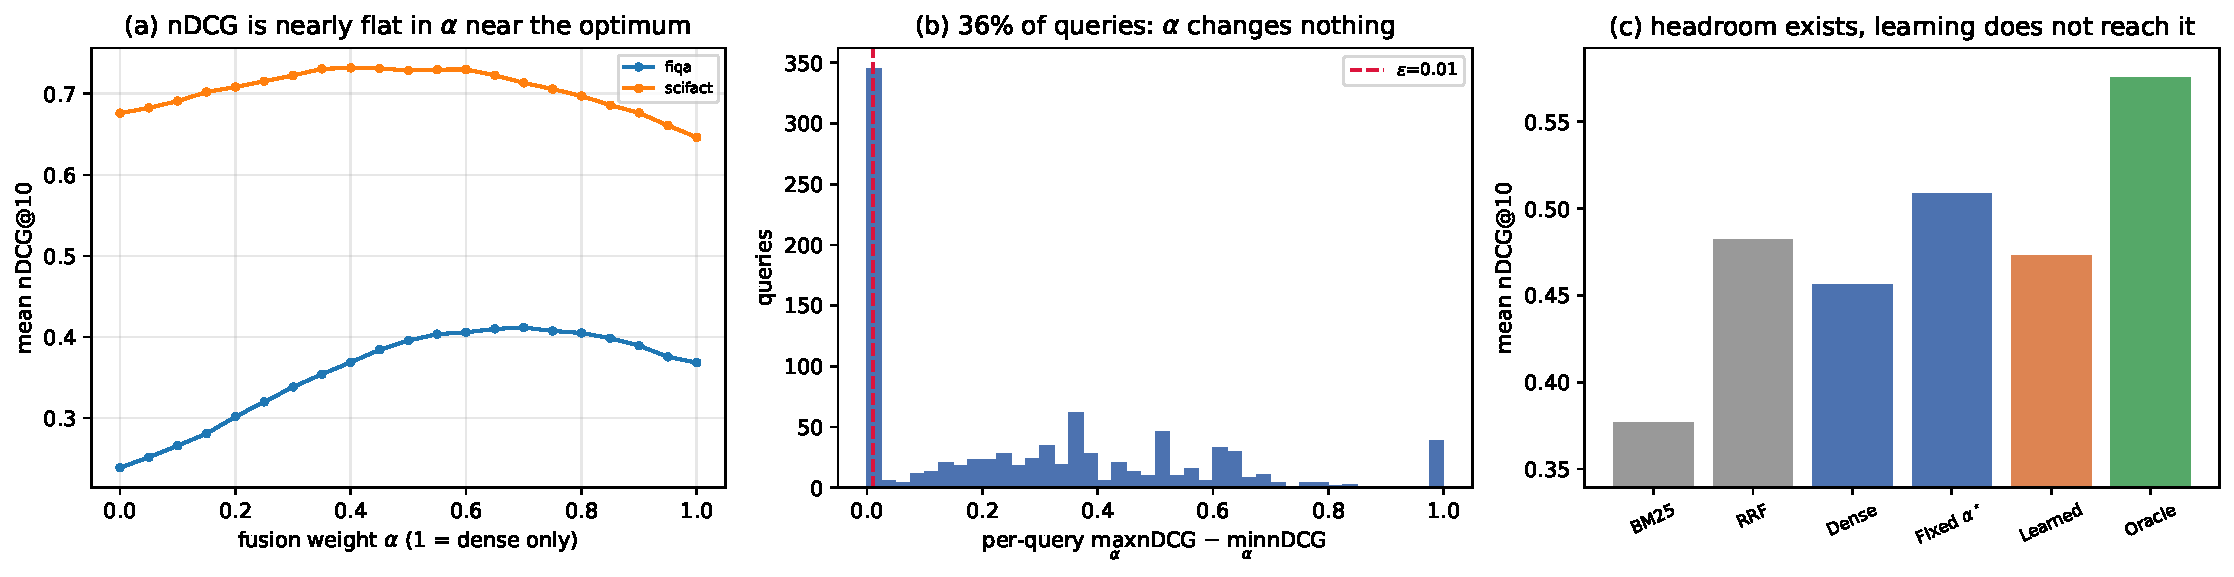
\includegraphics[width=\textwidth]{fig_alpha_headroom.pdf}
\caption{(a) Mean nDCG@10 as a function of the fusion weight $\alpha$, per
corpus: nearly flat near the optimum. (b) Distribution of the per-query range
$\max_\alpha \text{nDCG} - \min_\alpha \text{nDCG}$; the mass below $\epsilon$ is
the set of queries on which $\alpha$ is irrelevant. (c) Headroom: the oracle
sits well above the best fixed weight, and no learned policy approaches it.}
\label{fig:headroom}
\end{figure}

Table~\ref{tab:alpha_predictability} rules out the alternative explanation.
Cross-validated $R^2$ for predicting $\alpha^\star$ from the six features is
\alphaRtwo{}, and a gradient-boosting model with $500$ estimators does no better
than the small random forest --- capacity is not the constraint. A permutation
test places the achieved $R^2$ within the range obtained on shuffled labels.

\begin{table}[t]
\centering
\small
\caption{How predictable the oracle fusion weight is from the six query and score-distribution features, under 5-fold cross-validation.}
\label{tab:alpha_predictability}
\begin{tabular}{lccc}
\toprule
Model & CV $R^2$ & Spearman $\rho$ & MAE \\
\midrule
RandomForest(50,d5) [CIKM config] & 0.096 & 0.319 & 0.268 \\
RandomForest(500,d16) & 0.076 & 0.315 & 0.267 \\
GradientBoosting(500) & -0.078 & 0.271 & 0.279 \\
\bottomrule
\end{tabular}
\end{table}


We also evaluated two reformulations, on the grounds that regression onto a flat
target may simply be the wrong learning problem: a three-way router over
$\{\text{dense}, \text{RRF}, \text{lexical-leaning}\}$, and a selective policy
that deviates from dense only above a confidence threshold, traced as a
risk--coverage curve. Neither yields an interval excluding zero against
always-dense at any coverage level (Appendix~\ref{app:router}).

\paragraph{A note on the mechanism.} The implementation this study inherited
contained a rule that overrode the predictor with $\alpha = 1$ (pure dense)
whenever the maximum dense score exceeded $0.85$ or the BM25 coefficient of
variation fell below $0.1$. We report that variant separately in
Table~\ref{tab:main_retrieval}. Much of what such a system gains over naive
fusion comes from this rule --- that is, from declining to fuse --- rather than
from the learned weight. Isolating it is not a criticism of the idea so much as
a caution about where credit lands when a learned component sits behind a
hand-written guard.

\paragraph{Takeaway.} On modern dense retrievers evaluated at full corpus scale,
per-query fusion weighting is not worth deploying. The headroom is real, so the
problem is open; but it is bounded, and closing it requires a signal that
score-distribution statistics do not carry. Anyone attempting it should report
the oracle bound and the flatness distribution, because without them a null
result is indistinguishable from a weak predictor.

%% ===========================================================================
\section{RQ2: Do retrieval-layer defenses survive adaptive adversaries?}
\label{sec:rq2}
%% ===========================================================================

Poison documents are injected into a live BEIR corpus and must compete for
retrieval against real documents. Table~\ref{tab:attack_defense} is the main
result: attack success rate for every attacker against every defense, all at a
matched $1\%$ false-positive budget.

\begin{table}[t]
\centering
\small
\caption{Retrieval-level attack success rate at a matched false-positive budget of 1\%. Rows are attackers ordered by capability; columns are defenses ordered by cost. The \textit{none} column is the undefended payload-entry rate. Every defended cell is measured at the same operating point, calibrated on held-out clean documents.}
\label{tab:attack_defense}
\begin{tabular}{lcccccccc}
\toprule
Attacker & none & D1 & D1b & D2 & D3 & D4 & D5 & D6 \\
\midrule
A0\_static\_templates & 0.00 & 0.00 & 0.00 & 0.00 & 0.00 & 0.00 & 0.00 & 0.00 \\
A1\_query\_conditioned & 0.99 & 0.00 & 0.02 & 0.92 & 0.03 & 0.00 & 0.00 & 0.99 \\
A2\_imperative\_free & 1.00 & 0.99 & 1.00 & 0.74 & 0.02 & 0.00 & 0.22 & 1.00 \\
A3\_semantic\_camouflage & 1.00 & 1.00 & 1.00 & 0.98 & 0.99 & 0.99 & 1.00 & 1.00 \\
A4\_length\_matched & 1.00 & 1.00 & 1.00 & 0.98 & 0.68 & 0.00 & 0.66 & 1.00 \\
A5\_score\_guided & 1.00 & 1.00 & 1.00 & 0.98 & 0.68 & 0.05 & 0.15 & 1.00 \\
A6\_split\_payload & 1.00 & 1.00 & 1.00 & 0.98 & 0.93 & 0.01 & 0.90 & 1.00 \\
\bottomrule
\end{tabular}
\end{table}


\begin{figure}[t]
\centering
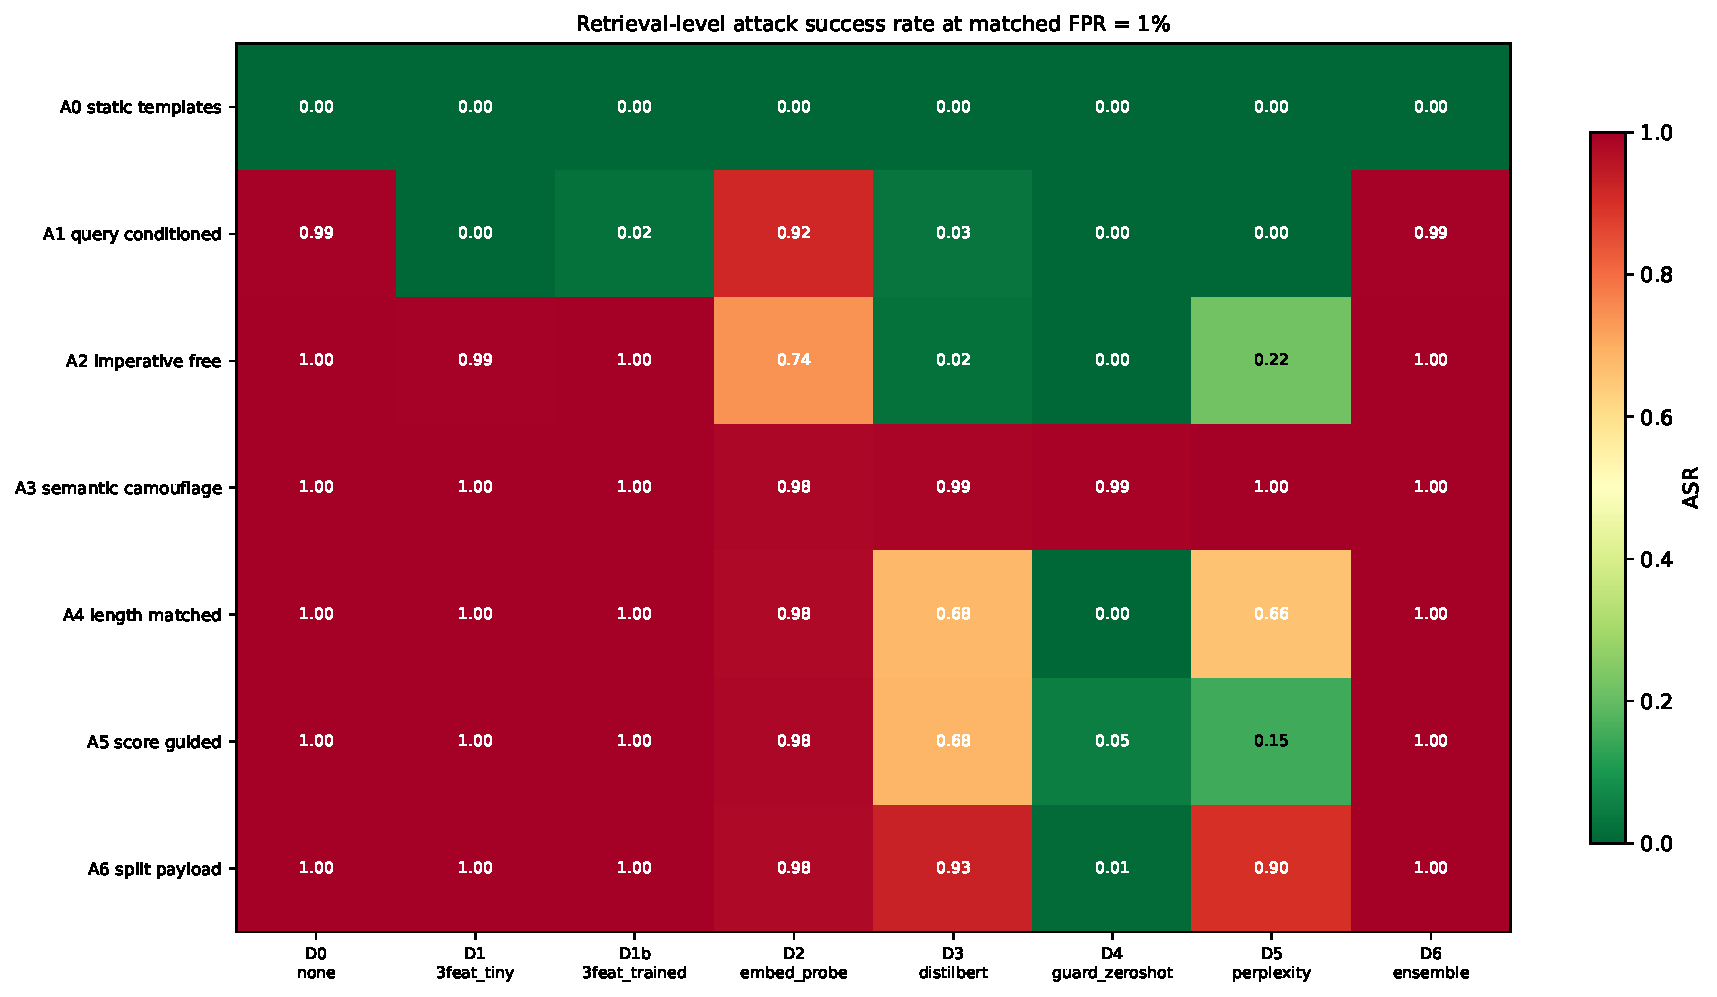
\includegraphics[width=0.86\textwidth]{fig_attack_defense_matrix.pdf}
\caption{Retrieval-level attack success at a matched $1\%$ false-positive
budget. Rows are attackers ordered by knowledge, columns are defenses ordered by
cost. Reading down a column shows how a defense degrades as the attacker learns
about it.}
\label{fig:matrix}
\end{figure}

Three things are visible in the matrix.

\paragraph{The lightweight filter holds only against attackers that do not
adapt.} D1 blocks static templates almost perfectly (ASR \asrDoneStatic{}) and
fails against A5 (ASR \asrDoneAdaptive{}). Each of its three features has an
evident counter, and the ladder applies them one at a time: A2 removes the
keywords, A3 raises centroid and query similarity by wrapping the directive in
genuine corpus text, A4 matches the clean length distribution. A5 needs to know
none of this specifically --- 200 queries to the detector suffice.

\paragraph{Training data is not the problem; the features are.} D1b uses the
same three features trained on thousands of real injection examples rather than
six templates, and does not close the gap. The three features are a lossy
summary of the document, and an attacker who controls the document controls the
summary. This distinction matters practically: it says the fix is not more
labels.

\paragraph{Capacity does help, at a cost.} D3 holds at \asrDthreeAdaptive{}
against A5 at the same operating point. That is a positive result, and it is
the one we would recommend acting on --- but it is a $66$M-parameter model
scoring every retrieved document, not three scalar features, and
Section~\ref{sec:cost} reports what that costs.

\paragraph{Utility.} Filtering blocks legitimate documents. At the $1\%$
operating point the cost is \utilityCost{} nDCG@10 on clean full-corpus
retrieval with no attack present (Table~\ref{tab:utility_cost}). Because this is
measured on the same corpora and metric as Section~\ref{sec:rq1}, the security
and utility numbers in this paper can be compared directly --- which was not
true of the earlier version, where the two came from different benchmarks with
different document distributions.

\paragraph{On the 99.3\% figure.} The earlier version reported that filtering
reduced adaptive-injection attack success from $99.3\%$ to $0.12\%$. Its
``adaptive'' attack was the target query's terms concatenated with a fixed
injection template; a document containing the query verbatim is retrieved
essentially always, so the $99.3\%$ is a property of the construction. Our A1
reproduces that attack and its undefended entry rate, reported alongside every
defended number in Table~\ref{tab:attack_defense}, so the reader can see what
the reduction is measured against. We include A1 rather than dropping it,
because the comparison between A1 and A5 in the same table is the clearest
statement of what changed.

%% ===========================================================================
\section{RQ3: How much does payload entry overstate risk?}
\label{sec:rq3}
%% ===========================================================================

Payload entry is a proxy. Table~\ref{tab:behavioural_gap} measures the quantity
it proxies for, on identical episodes: an instruction-tuned model reads the
retrieved context and we check whether it emits the canary. Episodes are built
from SQuAD \citep{rajpurkar2016squad}, so end-task quality is scorable with exact
match and token-$F_1$ alongside the security measurement.

\begin{table}[t]
\centering
\small
\caption{Retrieval-level payload entry versus downstream compliance, on the same episodes with no defense. The last column is the factor by which a retrieval-level metric must be discounted to estimate real exposure.}
\label{tab:behavioural_gap}
\begin{tabular}{llccc}
\toprule
Model & Attacker & ASR$_\text{retr}$ & ASR$_\text{behav}$ & $P(\text{comply}\mid\text{entry})$ \\
\midrule
Qwen2.5-1.5B-Instruct & A0\_static\_templates & 0.00 & 0.00 & -- \\
Qwen2.5-1.5B-Instruct & A1\_query\_conditioned & 0.99 & 0.00 & 0.00 \\
Qwen2.5-1.5B-Instruct & A2\_imperative\_free & 1.00 & 0.00 & 0.00 \\
Qwen2.5-1.5B-Instruct & A3\_semantic\_camouflage & 1.00 & 0.00 & 0.00 \\
Qwen2.5-1.5B-Instruct & A4\_length\_matched & 1.00 & 0.00 & 0.00 \\
Qwen2.5-1.5B-Instruct & A5\_score\_guided & 1.00 & 0.00 & 0.00 \\
Qwen2.5-1.5B-Instruct & A6\_split\_payload & 1.00 & 0.00 & 0.00 \\
Qwen2.5-3B-Instruct & A0\_static\_templates & 0.00 & 0.00 & -- \\
Qwen2.5-3B-Instruct & A1\_query\_conditioned & 0.99 & 0.00 & 0.00 \\
Qwen2.5-3B-Instruct & A2\_imperative\_free & 1.00 & 0.07 & 0.07 \\
Qwen2.5-3B-Instruct & A3\_semantic\_camouflage & 1.00 & 0.01 & 0.01 \\
Qwen2.5-3B-Instruct & A4\_length\_matched & 1.00 & 0.01 & 0.01 \\
Qwen2.5-3B-Instruct & A5\_score\_guided & 1.00 & 0.01 & 0.01 \\
Qwen2.5-3B-Instruct & A6\_split\_payload & 1.00 & 0.00 & 0.00 \\
\bottomrule
\end{tabular}
\end{table}


Conditioned on a payload reaching the context window, compliance is
\complianceRate{}. A retrieval-level metric therefore overstates exposure by
roughly \overstatement{}$\times$. This does not make retrieval-layer filtering
worthless --- the residual risk is real and the filter reduces it --- but it
does mean that a reported reduction in payload entry cannot be read as a
reduction in incidents, and no paper in this area that we are aware of, our own
earlier version included, reports the conversion factor.

\begin{figure}[t]
\centering
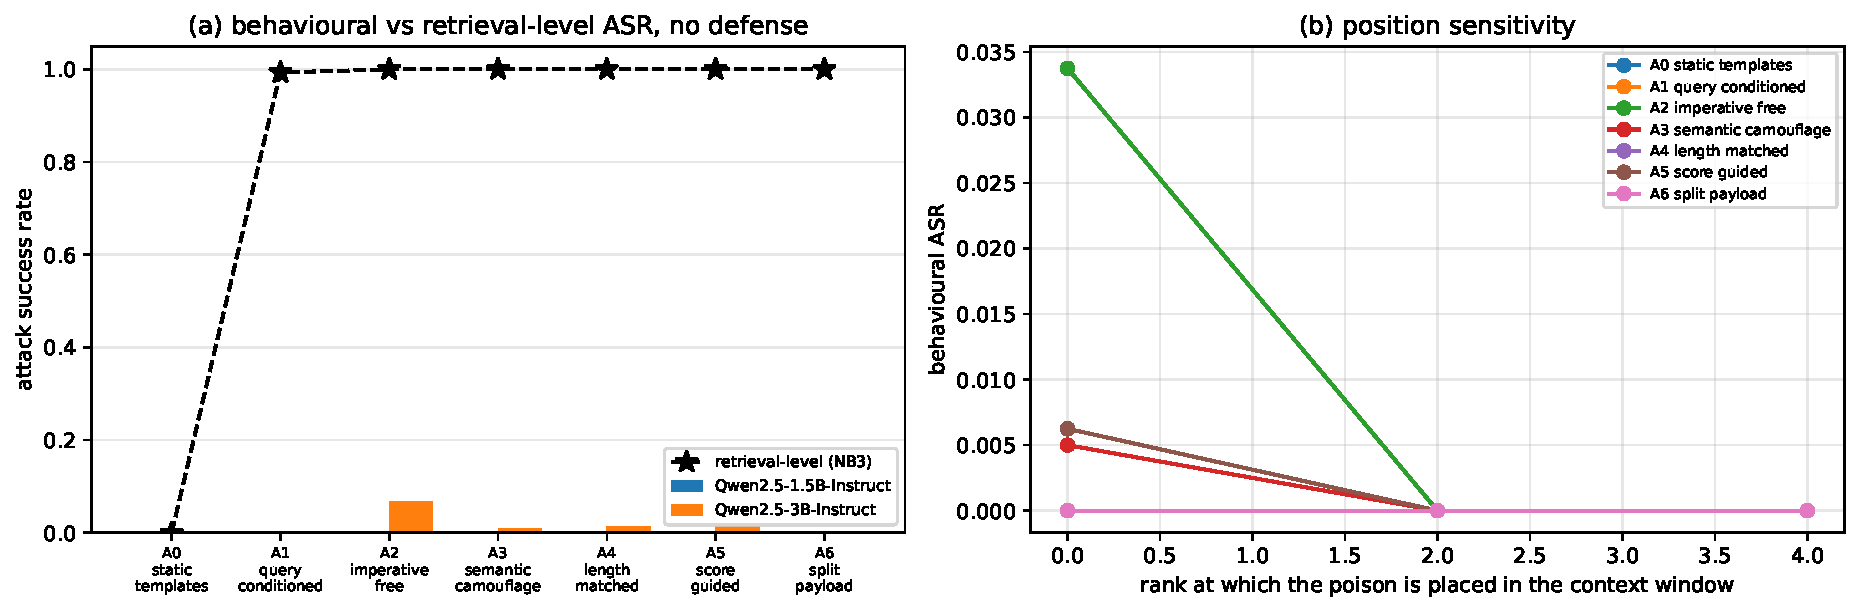
\includegraphics[width=\textwidth]{fig_behavioural_asr.pdf}
\caption{(a) Behavioural attack success versus retrieval-level payload entry
under no defense. The gap between the bars and the starred line is the
overstatement. (b) Compliance as a function of where the poison sits in the
context window.}
\label{fig:behavioural}
\end{figure}

\paragraph{Position matters.} Figure~\ref{fig:behavioural}(b) shows compliance
falling as the poison moves down the retrieved list, consistent with
\citet{liu2024lost}. A defense evaluated only on rank-0 injections reports its
hardest case; one evaluated on averages over positions reports something closer
to deployment. We report both.

\paragraph{Prompt hardening is a competitive baseline.} Adding two sentences to
the system prompt instructing the model to treat retrieved documents as data
rather than instructions reduces behavioural ASR to \promptHardenASR{}. This
costs nothing at retrieval time. Any retrieval-layer defense should be reported
against it, and the useful question is not whether filtering helps but whether
it catches what prompting misses. Our matrix answers that question for the
defenses we tested; we would encourage the same comparison elsewhere.

\paragraph{Tool selection.} We additionally run a tool-selection loop in which
the agent chooses one tool from an inventory and the attacker injects tool
documentation recommending an exfiltrating tool
(Table~\ref{tab:behavioural_gap}, lower block). This is a smaller-scale version
of the setting AgentDojo \citep{debenedetti2024agentdojo} evaluates thoroughly,
included because tool spoofing appears in this paper's threat model and a threat
model with an untested entry is a claim without evidence.

%% ===========================================================================
\section{What it costs}
\label{sec:cost}
%% ===========================================================================

Table~\ref{tab:cost} reports latency and quality from the same runs, on real
corpora with a persistent index, alongside cross-encoder forward passes per
query. We report forward passes because wall-clock on one GPU transfers to no
other machine, whereas forward passes do.

\begin{table}[t]
\centering
\small
\caption{Cost and quality from the same runs, on real corpora with a persistent index. Cross-encoder forward passes per query is the hardware-independent cost; latencies are on a single T4.}
\label{tab:cost}
\begin{tabular}{lrrrrrr}
\toprule
Corpus & $|D|$ & CE/query & nDCG@10 & p50 & p95 & p99 \\
\midrule
scifact & 5,183 & 0 & 0.760 & 40 & 44 & 46 \\
scifact & 5,183 & 10 & 0.738 & 79 & 83 & 86 \\
scifact & 5,183 & 50 & 0.722 & 246 & 261 & 264 \\
scifact & 5,183 & 100 & 0.720 & 463 & 487 & 495 \\
fiqa & 57,638 & 0 & 0.433 & 39 & 42 & 44 \\
fiqa & 57,638 & 10 & 0.417 & 76 & 80 & 83 \\
fiqa & 57,638 & 50 & 0.390 & 242 & 248 & 253 \\
fiqa & 57,638 & 100 & 0.386 & 447 & 461 & 465 \\
\bottomrule
\end{tabular}
\end{table}


The frontier in Figure~\ref{fig:cost} is the practical summary: reranking is
where both the quality and the latency are, filtering with a small transformer
adds a second per-document model pass over the top-$k$, and the fusion policy
costs and buys almost nothing. A system builder choosing where to spend should
read this figure and not the fusion table.

\begin{figure}[t]
\centering

\includegraphics[width=0.62\textwidth]{fig_cost_quality.pdf}
\caption{Cost/quality frontier of cross-encoder reranking on real corpora with a
persistent index, on a single T4.}
\label{fig:cost}
\end{figure}

%% ===========================================================================
\section{Discussion}
%% ===========================================================================

\paragraph{What we recommend reporting.} Three practices would change the
conclusions of much of this literature, and all three are cheap:

\begin{enumerate}
\item \textbf{Report ASR with its FPR.} An attack success rate without an
  operating point is not comparable to anything, including the same system in
  the same paper.
\item \textbf{Include at least one adaptive attacker.} The A5 attacker here is
  deliberately unsophisticated --- no gradients, a few hundred detector queries,
  edits any practitioner would think of. If a defense fails against that, the
  static numbers describe nothing.
\item \textbf{Report compliance given entry.} Payload entry is a legitimate
  intermediate metric, but the conversion factor to behaviour is what makes it
  actionable, and it can be measured with a 1.5B model in under an hour.
\end{enumerate}

\paragraph{What we would tell a system builder.} Spend on reranking, not on
fusion policy. If you deploy a retrieval-layer filter, use a fine-tuned
classifier rather than hand-designed features, calibrate it against your own
clean corpus rather than a published threshold, and treat it as one layer among
several --- our results suggest prompt-level mitigation is at least competitive
with it and composes with it at no retrieval cost.

\paragraph{On negative results.} Two of this paper's three findings are
corrective. We think they are more useful than the positive versions would have
been: a bounded negative result about per-query fusion tells the field where not
to spend effort and how much is actually on the table, and a demonstration that
lightweight filters fail adaptively is more actionable than another reported
two-order-of-magnitude reduction against static templates.

%% ===========================================================================
\section{Limitations}
%% ===========================================================================

\textbf{Retriever scale.} All encoders are small ($\leq$130M parameters), chosen
so the study runs end to end on a single commodity GPU. Whether the flatness of
the fusion objective persists for larger retrievers is untested, though we would
expect it to strengthen, since stronger dense retrievers leave less for the
lexical channel to add.

\textbf{Model scale in RQ3.} Compliance is measured on 1--3B instruction-tuned
models. Larger and better-aligned models plausibly comply less, which would make
the overstatement factor larger, not smaller; but the direction is an
expectation and not a measurement, and the absolute compliance rates should not
be transferred to frontier models.

\textbf{The adaptive attacker is weak by construction.} A5 uses no gradients and
a few hundred detector queries. A stronger attacker --- gradient-based, or with
white-box access to the detector's parameters --- would do better. Our numbers
are upper bounds on defense quality, not estimates of it.

\textbf{Single injection objective.} Compliance is measured against a canary-emission
directive. Exfiltration, refusal-induction, and multi-turn manipulation are
different objectives that may have different compliance profiles.

\textbf{English only, and one corpus for the security study.} The security
evaluation injects into a single BEIR corpus; absolute ASR depends on how hard
that corpus is to break into. The ordering across defenses is what we would
expect to transfer, not the absolute rates.

\textbf{No end-to-end agent.} RQ3 evaluates single-turn retrieval-then-answer and
single-step tool selection, not a multi-step agent with persistent state.
AgentDojo \citep{debenedetti2024agentdojo} covers that setting properly.

%% ===========================================================================
\section{Reproducibility}
\label{sec:repro}
%% ===========================================================================

Every experiment runs on a single free-tier GPU. The artifact contains six
notebooks corresponding to Sections~\ref{sec:rq1}--\ref{sec:cost}, each
independently runnable, each writing per-query results rather than aggregates.
Datasets are loaded at pinned revisions and all seeds are fixed. Attack
generation is deterministic: template selection uses a content digest rather
than Python's per-process randomised string hash, so the generated attack corpus
is byte-identical across runs, and it is released alongside the results.

Table generation is automated. The final notebook reads the artifacts, emits
every table in this paper, and writes \texttt{claims.json}, a record mapping each
numeric claim to the artifact that produced it; a checker then verifies that no
number in the manuscript is untraceable. This exists because the earlier version
of this work shipped tables that disagreed with each other and with its own
released logs, and neither we nor the reviewers had a mechanical way to catch it.

%% ===========================================================================
\section*{Acknowledgments}
%% ===========================================================================
Omitted for anonymous review.

\bibliographystyle{tmlr}
\bibliography{cognisync_tmlr}

\appendix

%% ===========================================================================
\section{Changes from the prior submission}
\label{app:changes}
%% ===========================================================================

This appendix exists so that a reader who has seen the earlier version can
locate every claim that changed.

\begin{table}[h]
\centering
\small
\caption{Claims that changed, and why.}
\begin{tabular}{p{0.29\textwidth}p{0.30\textwidth}p{0.33\textwidth}}
\toprule
Prior claim & Status & Where addressed \\
\midrule
$+2.80$ pp MRR@5 over dense retrieval &
Withdrawn. The comparison gave the proposed system a cross-encoder and the
baselines none. &
Section~\ref{sec:rq1}, matched-budget grid. \\
\addlinespace
MRR@5 $= 0.887$ on 29,011 query--passage pairs &
Withdrawn as a retrieval claim. The protocol reranked dataset-provided candidate
pools, so the value is not comparable to any published number. &
Section~\ref{sec:protocol}; all retrieval numbers are now full-corpus nDCG@10. \\
\addlinespace
Learned-$\alpha$ fusion is a contribution &
Reframed. It does not beat a tuned global weight; the contribution is the
oracle bound and the identifiability analysis. &
Section~\ref{sec:rq1}. \\
\addlinespace
Full-corpus result confirms the architecture scales (MRR@10 $0.9216$ vs $0.9197$) &
Withdrawn. The released script for that experiment used a fixed $\alpha = 0.6$
and no cross-encoder, so it did not evaluate the proposed system; and it ran on
train-split queries with positives appended to the index. &
Section~\ref{sec:rq1}, replaced by full BEIR. \\
\addlinespace
Filtering cuts adaptive-injection ASR from $99.3\%$ to $0.12\%$ &
Reframed. The $99.3\%$ was a property of an attack built to be retrieved; the
reduction does not survive an adapting attacker. &
Section~\ref{sec:rq2}, attacker ladder. \\
\addlinespace
Threshold sensitivity: FPR $0.0\%$ at every threshold &
Withdrawn. That table was computed on 16 hand-written query--document pairs and
disagreed with the paper's own $1.04\%$ FPR elsewhere. &
Section~\ref{sec:protocol}, single calibration procedure. \\
\addlinespace
$275.6$ ms average latency on a persistent 100K index &
Withdrawn. The measured corpus was generated from a 12-word vocabulary, and the
released logs record a different figure. &
Section~\ref{sec:cost}, real corpora with forward-pass counts. \\
\addlinespace
Episodic memory graph &
Removed. It was described but not implemented or evaluated. &
Section 2, noted as future work only. \\
\addlinespace
$86.36\%$ accuracy on \texttt{deepset/prompt-injections} &
Retained as a component result, and superseded: that number is a
single-operating-point accuracy on a small corpus. &
Section~\ref{sec:rq2} reports ROC-AUC and matched-FPR ASR instead. \\
\bottomrule
\end{tabular}
\end{table}

%% ===========================================================================
\section{Fusion feature definitions and fitting protocol}
\label{app:features}
%% ===========================================================================

\paragraph{Normalisation.} Let $D$ and $L$ be the top-$m$ lists from the dense
and lexical channels. Scores are min--max normalised within each list; if a
list's scores are constant, all normalised values are set to $0$. The fused
candidate set is $D \cup L$, and a document in $D \setminus L$ receives
$\tilde{s}_{\text{lex}} = 0$ (symmetrically for $L \setminus D$). We use
$m = 1000$ throughout.

\paragraph{Features.} The six features predicting $\alpha$ are: query length in
whitespace tokens; the standard deviation of the normalised dense scores; the
standard deviation of the normalised lexical scores; the coefficient of
variation of each (set to $0$ when the corresponding mean is $0$); and a binary
indicator for identifier-like queries, which fires on an explicit
\texttt{id}/\texttt{uuid}/\texttt{hash}/\texttt{key}/\texttt{sha}/\texttt{md5}
token, a hex literal of four or more digits, a dotted version string, or an
alphanumeric run of sixteen or more characters.

\paragraph{Fitting.} $\alpha$ is fit once on $3{,}000$ MS MARCO
\citep{nguyen2016msmarco} training queries
against a $200{,}000$-passage corpus and applied unchanged to every BEIR
collection --- a zero-shot transfer protocol. The oracle target is the grid
point in $\{0.00, 0.05, \ldots, 1.00\}$ maximising nDCG@10. The global
$\alpha^\star$ baseline is the grid point maximising \emph{mean} nDCG@10 on the
same fitting set. No BEIR test query is used for fitting.

%% ===========================================================================
\section{Router and selective-deviation results}
\label{app:router}
%% ===========================================================================

Regression onto a flat target may be the wrong formulation, so we evaluated two
alternatives on the same features. The router is a three-way classifier over
$\{\text{dense}, \text{RRF}, \alpha{=}0.3\}$ with the label being whichever wins
per query. The selective policy ranks by dense unless the router's confidence
exceeds a threshold, and we sweep the threshold to trace coverage against
benefit. Full curves are in the released artifact
(\texttt{nb2\_risk\_coverage.csv}); no threshold yields a bootstrap interval
excluding zero against always-dense.

%% ===========================================================================
\section{Attack corpus}
\label{app:attacks}
%% ===========================================================================

The generated attack documents are released in full
(\texttt{nb3\_attack\_documents.parquet} and, for the adaptive attacker,
\texttt{nb3\_a5\_documents.parquet}). Each A5 record carries the final detection
score, the number of detector queries consumed, and whether the document ended
below the deployed threshold, so the optimisation can be audited rather than
taken on trust. Section~\ref{sec:rq3} replays these exact documents through the
language models, which is what establishes that evasion did not come at the cost
of the payload ceasing to work.

\end{document}
